\newpage
\section{Ergebnisse}\label{sec:ergebnisse}
\subsection{Benutzungsoberfläche des RAG-Chatbots}\label{subsec:benutzungsoberflache-des-rag-chatbots}
Abbildung~\ref{fig:rag-chatbot-ui} zeigt die Benutzungsoberfläche des prototypischen RAG-Chatbots, wie sie im Webbrowser dargestellt wird.
\vspace{1cm}
\FloatBarrier
\begin{figure}[H]
    \centering
    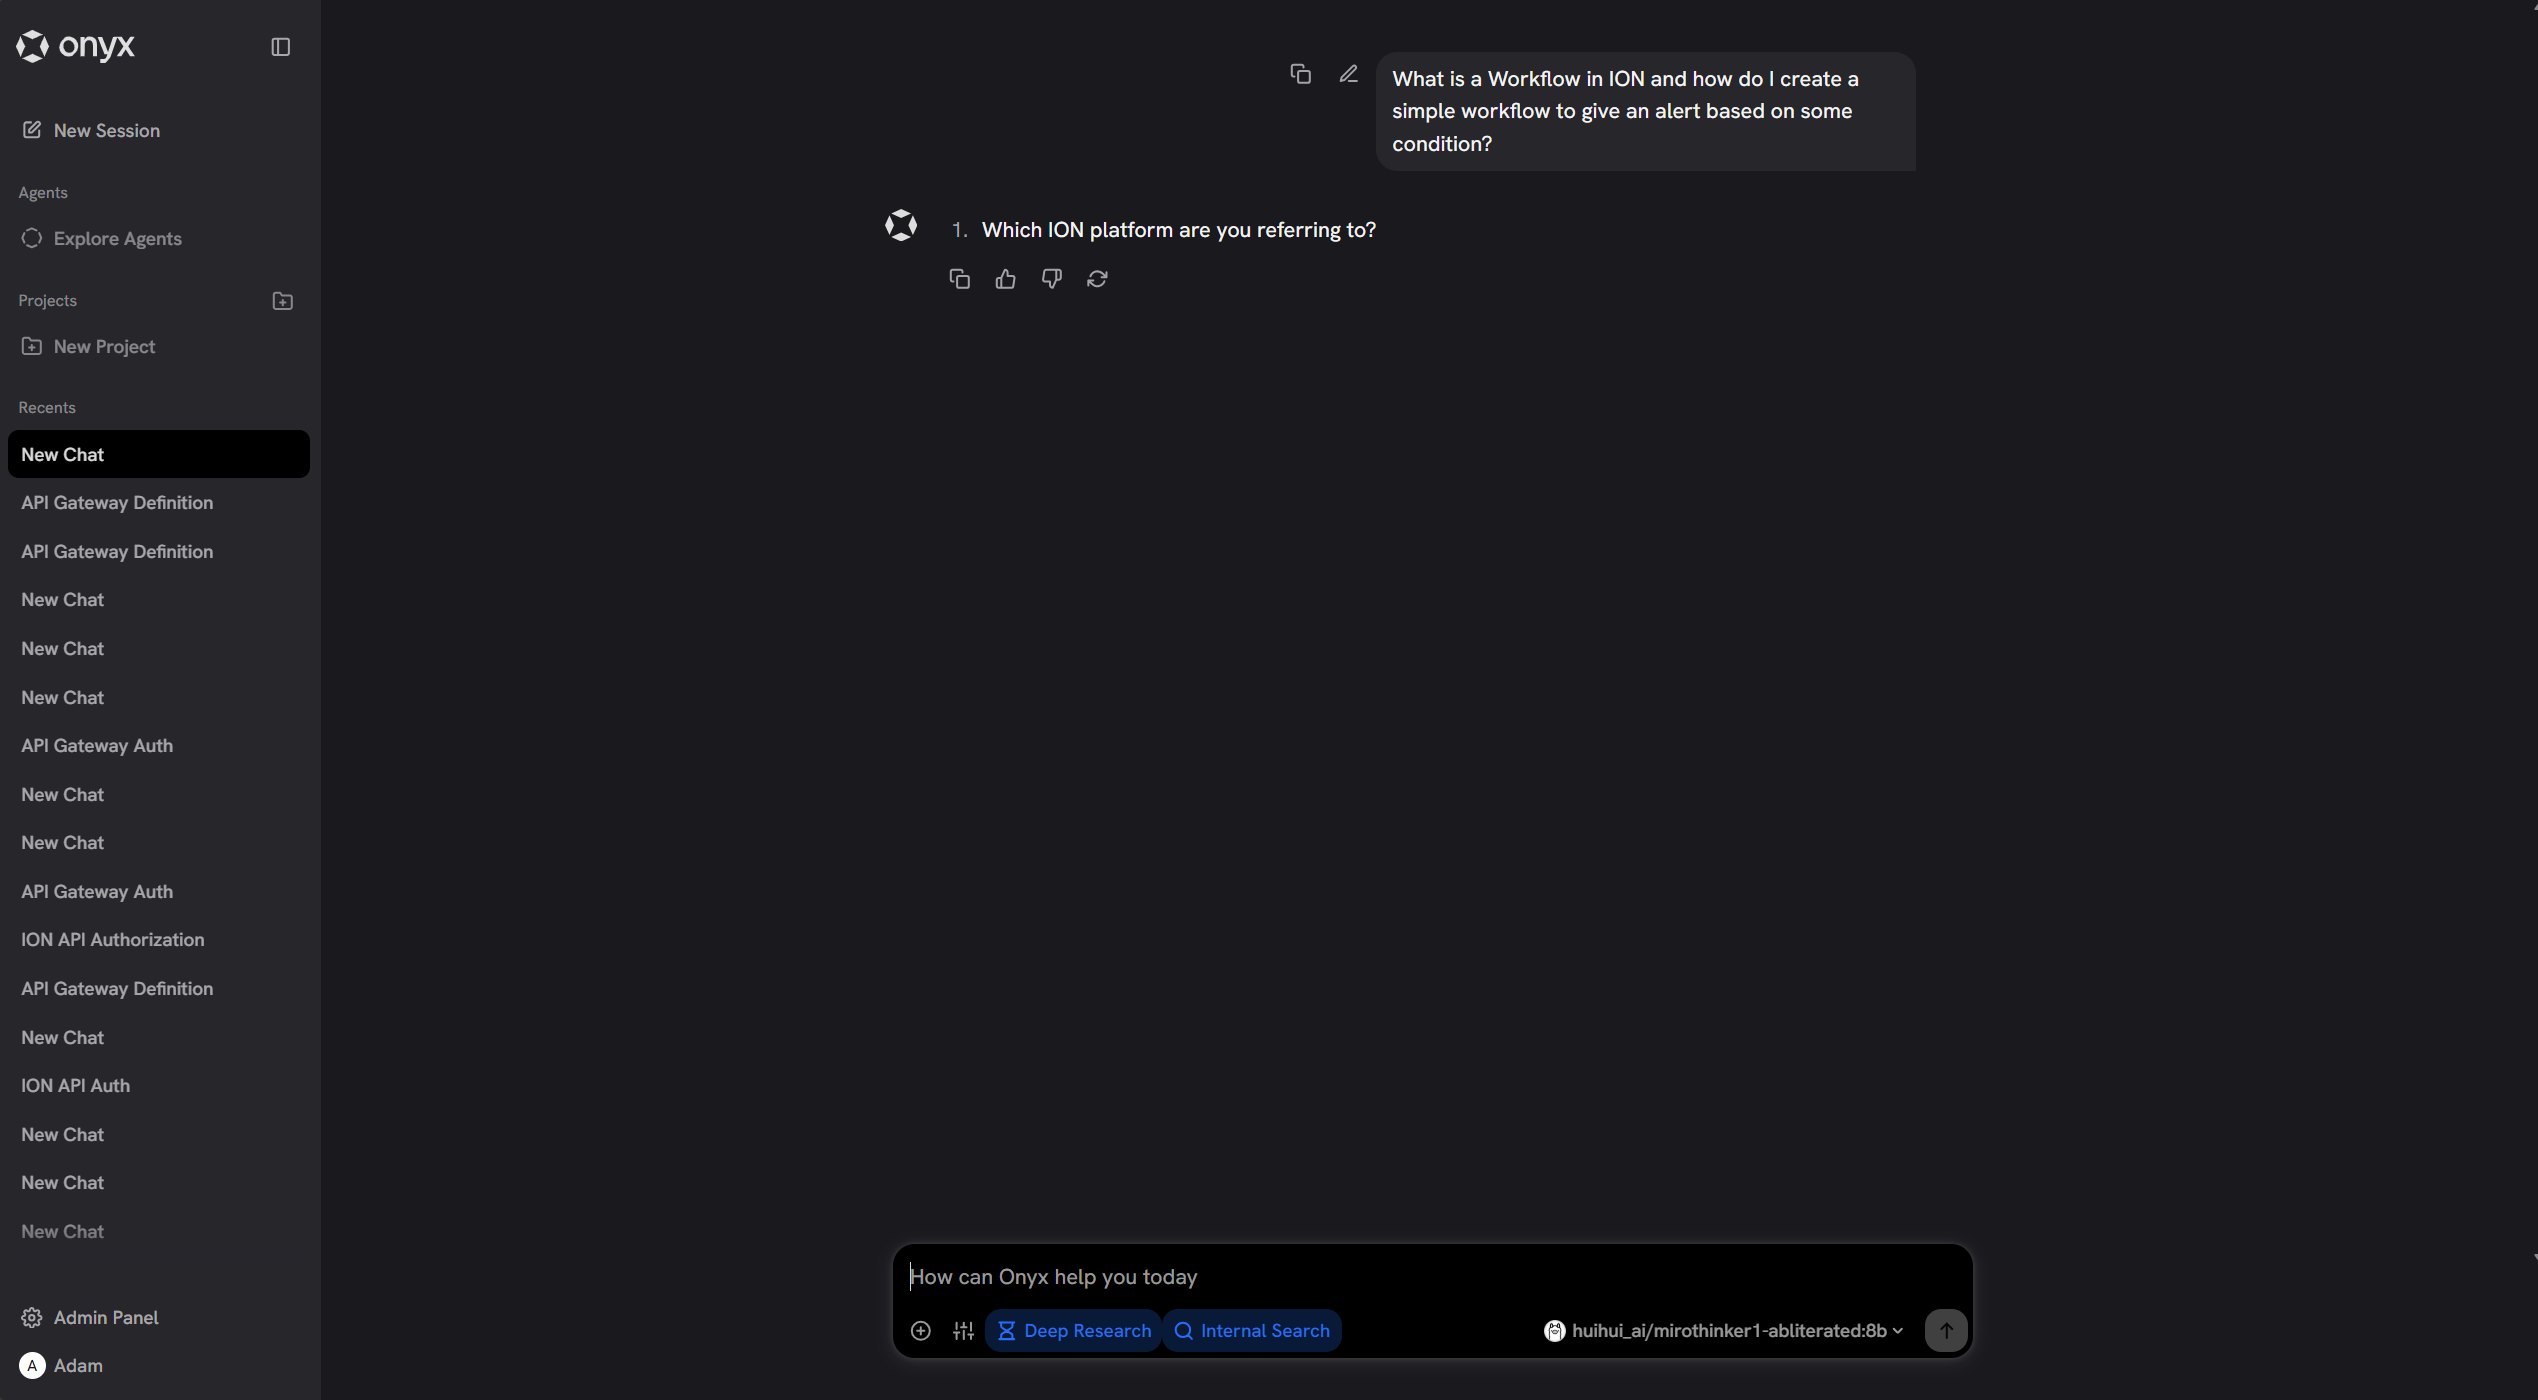
\includegraphics[width=1\textwidth]{Bilder/Onyx Interface}
    \caption{Benutzungsoberfläche des RAG-Chatbots im Webbrowser}
    \label{fig:rag-chatbot-ui}
\end{figure}
\FloatBarrier
\vspace{1cm}
Die Oberfläche ist in drei Hauptbereiche gegliedert:
\begin{itemize}
    \item \textbf{Linke Seitenleiste:} Hier befinden sich Navigationselemente für verschiedene Funktionen des Chatbots, wie z.\,B.\ das Starten neuer Chats, das Anzeigen von Chat-Verläufen und das Zugreifen auf Einstellungen.
    \item \textbf{Hauptchatbereich:} In der Mitte wird der eigentliche Chatverlauf angezeigt. Nutzeranfragen und Chatbot-Antworten werden chronologisch dargestellt, wobei jede Antwort des Chatbots mit Quellenverweisen auf die verwendeten Dokumente versehen ist.
    \item \textbf{Eingabefeld:} Am unteren Rand befindet sich das Eingabefeld, in das Nutzer ihre Fragen oder Anfragen eingeben können. Ein Senden-Button ermöglicht das Abschicken der Anfrage an den Chatbot.
\end{itemize}

Damit bietet die Oberfläche eine intuitive und benutzerfreundliche Möglichkeit, mit dem RAG-Chatbot zu interagieren und auf das interne Wissen der Organisation zuzugreifen.

\subsection{Ausgangslage und Zielsetzung der Arbeit}\label{subsec:ausgangslage-und-zielsetzung-der-arbeit}

Diese Masterarbeit ist aus einer sehr praktischen Problemstellung heraus entstanden: In der Organisation liegen zentrale Informationen in Microsoft~365-Diensten (insbesondere SharePoint und OneDrive) sowie in weiteren heterogenen Quellen vor, jedoch ist dieses Wissen im Arbeitsalltag nur mit hohem Zeitaufwand nutzbar.
Die in Abschnitt~\ref{sec:problemanalyse} herausgearbeitete Ist-Situation ist durch eine Kombination aus Informationsüberlastung, verstreuten Wissensartefakten, uneinheitlicher Dokumentqualität und begrenzter Suchunterstützung geprägt.
Die klassische Volltextsuche liefert zwar Trefferlisten, aber selten diejenige konsolidierte, nachvollziehbare Antwort, die Mitarbeitende in zeitkritischen Situationen benötigen.
Gleichzeitig scheiden Cloud-basierte LLM-Dienste für viele Anwendungsfälle aus Datenschutz- und Compliance-Gründen aus, da sensible Inhalte die Unternehmensumgebung nicht verlassen dürfen.

Vor diesem Hintergrund war das übergeordnete Ziel, die technische Machbarkeit und den praktischen Nutzen eines datenschutzkonformen, vollständig on-premises betriebenen RAG-Chatbots zu untersuchen.
Dabei standen zwei Leitfragen im Zentrum: (1) ob sich eine solche Lösung mit Open-Source-Werkzeugen in einer überwiegend Windows-dominierten IT-Realität eines kleineren Unternehmens umsetzen lässt, und (2) ob ein solcher Chatbot gegenüber der bestehenden Dokumentensuche einen messbaren bzw.\ plausibel begründbaren Mehrwert liefert, ohne neue Risiken in Bezug auf Datenschutz, Sicherheit und Betrieb einzuführen.
Die in Abschnitt~\ref{sec:einleitung} formulierten Forschungsfragen und Ziele dienten als strukturierender Rahmen und werden im Folgenden zusammengeführt und beantwortet.

\subsection{Zusammenführung der Ergebnisse entlang der Forschungsfragen}\label{subsec:zusammenfuhrung-der-ergebnisse-entlang-der-forschungsfragen}

\subsubsection{Forschungsfrage 1: Technische Umsetzung im gegebenen IT-Umfeld}

Die Arbeit zeigt, dass ein RAG-Chatbot für firmeninterne Wissensbasen im beschriebenen Umfeld grundsätzlich realisierbar ist, sofern einige technische Randbedingungen eingehalten werden.
Die wesentliche Architekturentscheidung bestand darin, die RAG-Pipeline in klar abgegrenzte Komponenten zu zerlegen (Connectoren, Parsing, Chunking, Embeddings, Vektorsuche, Retrieval, LLM-Inferenz und Chat-Interface) und diese in einer containerisierten Umgebung zu betreiben.
Diese Modularisierung ist nicht nur ein akademisches Architekturideal, sondern erwies sich in der Umsetzung als praktische Voraussetzung, um Engpässe diagnostizieren und zielgerichtet beheben zu können (vgl.\ Abschnitt~\ref{sec:technische-umsetzung}).

Als technische Grundlage wurde Onyx (ehemals Danswer) als Plattform gewählt, weil es zentrale Anforderungen in einer integrierten Lösung adressiert: Anbindung typischer Unternehmensquellen über Connectoren, Indexierungs- und Retrieval-Mechanismen, eine administrierbare Oberfläche sowie die Möglichkeit, ein lokales LLM-Backend einzubinden.
Die Auswahl wurde in der Problemanalyse über ein gewichtetes Bewertungsmodell begründet (Tabelle~\ref{tab:rag-tools-gewichtung}) und damit nachvollziehbar an den zuvor hergeleiteten Qualitätszielen ausgerichtet (Abschnitt~\ref{subsec:zielbild}).

Für die lokale Modellinferenz wurde Ollama als Laufzeit eingesetzt und in die Onyx-Umgebung integriert.
Damit konnte die zentrale Datenschutzanforderung technisch stringent umgesetzt werden: Nutzeranfragen, Dokumentkontexte und generierte Antworten verbleiben innerhalb der lokalen Infrastruktur, ohne dass Inhalte an externe Cloud-APIs übertragen werden.
Die Schnittstelle zwischen RAG-Plattform und Modelllaufzeit erwies sich dabei als kritischer Stabilitätsfaktor.
Die in der ersten Instanzierung aufgetretenen Timeouts in der litellm-basierten Kommunikation machen deutlich, dass produktionsnahe Robustheit nicht allein aus der Wahl der Komponenten folgt, sondern aus deren konkreter Parametrisierung, Versionskonstellation und Betriebsumgebung.
Die pragmatische Entscheidung, Timeouts im Onyx-Wrapper fest zu verdrahten, erhöhte die Stabilität der prototypischen Instanz, stellt jedoch zugleich einen bewussten Wartbarkeitskompromiss dar: Für spätere Upstream-Updates ist dieser Eingriff eine potentielle Konfliktstelle, die entweder sauber über Konfigurationen aufzulösen oder als Patch-Strategie organisatorisch abzusichern wäre.

Ein weiteres zentrales Ergebnis betrifft die Hardwarebasis.
Die anfängliche Hypothese, eine rein CPU-basierte Inferenz könne für ein Kleinunternehmen eine ausreichend günstige, wartbare und praktikable Grundlage bilden, ließ sich in den Experimenten nicht bestätigen.
Die beobachteten Antwortzeiten auf CPU (bis in den Minutenbereich selbst für triviale Eingaben) führten zu einer qualitativ schlechten Nutzererfahrung und zu fehlender Skalierbarkeit im Mehrnutzerbetrieb.
Damit wurde GPU-Unterstützung zu einer praktischen Voraussetzung für das Systemziel \glqq Antwort in wenigen Sekunden\grqq{} (vgl.\ NFA1).
Die Arbeit zeigt zugleich, dass GPU-Unterstützung nicht zwangsläufig einen klassischen Server oder Enterprise-Hardware erfordert: Ein leistungsfähiges Consumer-Notebook mit dedizierter GPU kann als kosteneffiziente Plattform für einen Prototyp bzw.\ Pilotbetrieb dienen, sofern dessen Ressourcenprofil (VRAM, RAM, TGP, Kühlung, Dauerlastfähigkeit) zum Modell- und Nutzungsprofil passt.

Zusammenfassend beantwortet die Arbeit Forschungsfrage~1 damit wie folgt:
Eine technische Umsetzung ist möglich, wenn (a) RAG-Plattform und LLM-Laufzeit strikt lokal betrieben werden, (b) Connectoren und Dokumentpipelines robust für heterogene Office-Formate konfiguriert sind, (c) GPU-Ressourcen eingeplant werden, und (d) kritische Betriebsparameter wie Timeouts, Chunking- und Retrieval-Konfigurationen empirisch auf die realen Laufzeiten abgestimmt werden.

\subsubsection{Forschungsfrage 2: Mehrwerte gegenüber klassischen Suchsystemen}

Der wesentliche Mehrwert eines RAG-Chatbots liegt nicht darin, \emph{mehr} Dokumente zu finden, sondern darin, den Schritt von der Trefferliste zur nutzbaren Antwort zu verkürzen.
Die Baseline über SharePoint/OneDrive liefert typischerweise Dokumente, während der Chatbot Passagen aggregiert, verdichtet und in eine anwendernahe Antwortform bringt (vgl.\ Abschnitt~\ref{sec:evaluation}).
In den beschriebenen Szenarien zeigte sich der Vorteil insbesondere dort, wo Informationen über mehrere Dokumente verteilt sind oder in umfangreichen Dokumenten tief eingebettet liegen.
Die Rollenperspektive aus der Problemanalyse hilft, diesen Effekt zu erklären:
Projektmanager benötigen häufig prozess- und richtlinienbezogene Antworten, bei denen einzelne Schlüsselstellen in QM- oder Prozessdokumenten relevant sind.
Anwendungsberater benötigen konsistente, dokumentgetreue Aussagen zu Produktfunktionen oder Konfigurationsschritten, die oft über Release-Notes, Handbücher und interne Best-Practice-Dokumente verteilt sind.
Technische Berater profitieren besonders, wenn Troubleshooting-Schritte und Konfigurationshinweise aus mehreren technischen Quellen zusammengeführt werden.

Die in der Evaluation beschriebene Tabelle zum Vergleich von SharePoint-Suche und RAG-Chatbot (Tabelle~\ref{tab:vergleich_sp_rag}) illustriert diesen Mehrwert qualitativ:
Der Chatbot verkürzt die Suchzeit, reduziert die Anzahl notwendiger Dokumentöffnungen und erhöht die Nachvollziehbarkeit durch Quellenverweise.
Gerade die Kombination aus komprimierter Antwort und Rückverweis auf Dokumentstellen adressiert ein Kernproblem klassischer Suchsysteme: Die kognitive Last wird reduziert, ohne den Zugriff auf die Primärquelle zu verlieren.

Gleichzeitig wurde ein wichtiges Gegenresultat sichtbar:
Der Mehrwert ist stark abhängig von der Qualität der Wissensbasis und deren maschineller Verarbeitbarkeit.
Sobald entscheidende Informationen primär in Tabellen, Screenshots, schlecht strukturierten Legacy-Dokumenten oder unzureichend gepflegten Inhalten vorliegen, sinkt die Antwortqualität oder der Chatbot muss auf allgemeine Aussagen ausweichen.
Damit bestätigt die Arbeit eine praxisrelevante Schlussfolgerung:
RAG ist kein Ersatz für Wissensmanagement, sondern ein Verstärker gut gepflegter Dokumentation.
Die Produktivitätsgewinne entstehen dort, wo Dokumente ausreichend strukturierte, extrahierbare Information enthalten und wo der Index diese Information zuverlässig auffindbar macht.

In der Zusammenschau beantwortet die Arbeit Forschungsfrage~2 damit wie folgt:
Ein RAG-Chatbot bietet gegenüber klassischer Suche vor allem dann Mehrwert, wenn Fragen über mehrere Dokumente hinweg beantwortet werden müssen, wenn relevante Passagen schwer auffindbar sind, und wenn Nachvollziehbarkeit über Zitationen/Links gewährleistet wird.
Wo Dokumentqualität oder Extraktionsfähigkeit niedrig sind, reduziert sich dieser Mehrwert deutlich und kann im Extremfall in Frustration umschlagen.

\subsubsection{Forschungsfrage 3: Faktoren für Qualität und Akzeptanz im Unternehmenskontext}

Die Qualität und Akzeptanz des Chatbots wurde in der Arbeit nicht als \glqq Eigenschaft des Modells\grqq{}, sondern als Ergebnis eines Zusammenspiels mehrerer Schichten sichtbar.
Vier Faktoren erwiesen sich als besonders prägend.

Erstens ist die Dokumentqualität ein dominanter Einflussfaktor.
Unklare Struktur, Übersetzungsartefakte, inkonsistente Terminologie und schwer extrahierbare Inhalte wirken direkt auf das Retrieval und damit auf die Kontextgrundlage der Antwort.
Dies betrifft insbesondere die in der Problemanalyse erwähnten technischen Dokumente für Infor LN/OS, die häufig heterogene Autorenstile und Formatierungen aufweisen.
Damit entsteht eine konkrete, organisatorische Implikation: Ein RAG-System erzeugt nicht automatisch \glqq saubere\grqq{} Antworten aus \glqq unsauberen\grqq{} Dokumenten; vielmehr wird die Verbesserung der Dokumentationsqualität selbst zu einer indirekten, aber wirksamen Stellschraube für die Systemqualität.

Zweitens ist die Retrieval- und Chunking-Konfiguration entscheidend.
Zu große Chunks erhöhen die Wahrscheinlichkeit, irrelevanten Kontext zu injizieren; zu kleine Chunks zerschneiden Zusammenhänge und reduzieren die Fähigkeit, komplexe Fragen mit konsistentem Kontext zu beantworten.
Zwar wäre eine abschnittsbasierte Chunking-Strategie ideal, doch Onyx gibt dies derzeit nicht her.
Eine Anpassung der Software wäre hier ein möglicher Ausbaupfad, der aber über den Rahmen der Arbeit hinausgeht.
Akzeptanzseitig ist aber weiterhin relevant, dass Antworten konsistent und reproduzierbar wirken.
Wenn das Retrieval stark schwankt oder häufig nur teilweise relevante Passagen liefert, sinkt das Vertrauen.
Daraus folgt: Die Akzeptanz hängt weniger davon ab, ob einzelne Antworten \glqq beeindruckend\grqq{} sind, sondern ob sie im Alltag verlässlich sind.

Drittens beeinflusst die Modellwahl das Verhältnis von Antwortqualität, Tool-Kompatibilität und Latenz.
Die ersten Tests zeigen, dass eine bloße Erhöhung der Parameteranzahl nicht automatisch zu einem besseren Gesamtsystem führt, wenn dadurch Antwortzeit und Stabilität leiden.
Das beobachtete instabile Antwortverhalten bei größeren Modellen sowie die Schwierigkeiten eines spezialisierten ChatQA-Modells im Zusammenspiel mit toolbasierter Agentenlogik unterstreichen, dass \glqq RAG-Tauglichkeit\grqq{} nicht allein über Benchmarks oder Marketingbegriffe beurteilt werden kann.
Ein Modell kann im statischen Kontext-QA gut sein und dennoch im agentischen Workflow (Retrieval anstoßen, Tool-Ausgaben interpretieren, Antwort strukturieren) versagen.
Für die Praxis bedeutet dies: Modellwahl ist ein integrativer Designschritt, der Prompting, Agentenlogik, Laufzeitumgebung und Retrieval-Design zusammen denken muss.

Viertens ist die Antwortzeit ein Akzeptanzkriterium, das in der Praxis stärker wirkt als viele inhaltliche Nuancen.
Die Evaluation beschreibt für GPU-gestützte Inferenz Antwortzeiten, die subjektiv als flüssig wahrgenommen wurden, während CPU-basierte Antworten inakzeptabel lange dauerten.
Damit wird die nicht-funktionale Anforderung NFA1 nicht als \glqq technische Kennzahl\grqq{} sichtbar, sondern als Akzeptanzschwelle: Wird sie nicht erfüllt, wird das System unabhängig von inhaltlichen Qualitäten nicht genutzt.

Zusammenfassend beantwortet die Arbeit Forschungsfrage~3 damit wie folgt:
Die Akzeptanz eines RAG-Chatbots hängt im Unternehmenskontext primär von Verlässlichkeit (Retrieval-Qualität, stabile Prompts, konsistente Antworten), Nachvollziehbarkeit (Zitationen/Links), Antwortzeit (Sekundenbereich) und der Qualität der Wissensbasis ab.
Die Modellwahl ist wichtig, aber nicht isoliert entscheidend; sie muss im Zusammenspiel mit Agentenlogik und Infrastruktur betrachtet werden.

\subsubsection{Forschungsfrage 4: Herausforderungen bei Datenschutz, Sicherheit und Integration}

Aus Datenschutzperspektive zeigt die prototypische Architektur eine klare, wirksame Grundentscheidung:
Sämtliche Verarbeitung bleibt lokal; es werden keine Inhalte an Drittanbieter übertragen.
Damit wird die zentrale Anforderung der Datenresidenz praktisch umgesetzt.
Gleichzeitig wurde deutlich, dass Datenschutzkonformität im Unternehmenskontext nicht allein durch \glqq On-Premises\grqq{} erfüllt ist.
Zwei Herausforderungen bleiben zentral.

Erstens ist die Berechtigungsdurchsetzung technisch und organisatorisch anspruchsvoll.
Onyx bietet prinzipiell Mechanismen, Berechtigungsstrukturen aus Quellsystemen zu spiegeln, doch die Evaluation benennt, dass eine vollständige Anbindung an Entra ID/Active Directory im Rahmen der Arbeit noch nicht umgesetzt wurde.
Damit ist das Need-to-know-Prinzip im Prototyp zwar konzeptionell adressiert, aber in der Praxis noch nicht durchgängig abgesichert.
Für einen produktiven Einsatz wäre dies ein zentraler Ausbaupfad, weil gerade im M365-Kontext feingranulare Berechtigungen und Gruppenstrukturen entscheidend für Compliance sind.

Zweitens verschiebt ein RAG-System die Angriffsfläche:
Neben klassischen Infrastrukturrisiken treten LLM-spezifische Risiken wie Prompt Injection über Dokumentinhalte, Datenvergiftung des Korpus oder ungewollte Offenlegung sensibler Inhalte in Antworten.
Die Arbeit hat diese Risiken in den Anforderungskriterien explizit berücksichtigt (u.\,a.\ Sicherheitsfunktionen, Logging/Monitoring), jedoch sind daraus im Prototyp noch keine vollständig formalisierten Schutzmechanismen (z.\,B.\ policybasierte Output-Filter, systematisches Red-Teaming, dokumentbasierte Sanitization-Pipelines) abgeleitet.
Der Prototyp adressiert das Risiko vor allem über die restriktive Agenteninstruktion, die Kontextbindung und die Deaktivierung externer Websuche.
Das ist ein wirksamer erster Schritt, ersetzt aber keine ganzheitliche Sicherheitsarchitektur.

In der Integrationsdimension zeigte die Arbeit, dass ein lauffähiger Pilotbetrieb ohne tiefgreifende Eingriffe in die bestehende Systemlandschaft möglich ist, sofern ein Web-Frontend als Einstiegspunkt gewählt wird.
Die Offenheit für weitere Kanäle (Teams, REST-Integration) ist architektonisch vorbereitet.
Der Aufwand verschiebt sich jedoch, sobald Enterprise-Integrationen (SSO, Audit-Logging, zentrale Monitoring-Stacks, Lifecycle-Management) gefordert sind.
Damit ergibt sich ein realistisches Bild: Ein Prototyp ist mit überschaubarem Aufwand möglich; ein produktionsreifer Rollout benötigt zusätzliche organisatorische und technische Reifegrade, insbesondere in Identity, Governance und Betrieb.

Zusammenfassend beantwortet die Arbeit Forschungsfrage~4 damit wie folgt:
On-Premises-Betrieb reduziert zentrale Datenschutzrisiken, erzeugt aber neue Anforderungen an Berechtigungsspiegelung, LLM-spezifische Sicherheit (Prompt Injection etc.) und revisionsfähigen Betrieb.
Die größte offene Integrationsbaustelle im Prototyp ist die durchgängige Anbindung an bestehende Identity- und Berechtigungssysteme.

\subsection{Rückschluss auf die Ziele der Arbeit}\label{subsec:ruckschluss-auf-die-ziele-der-arbeit}

Die in der Einleitung formulierten Ziele lassen sich wie folgt bilanziell zusammenführen.

Der Prototyp eines RAG-Chatbots, der interne Dokumente aus SharePoint und OneDrive nutzt, konnte konzeptionell und prototypisch umgesetzt werden.
Die Pipeline von Dokumentingestion, Parsing, Chunking, Vektorisierung, Retrieval und Antwortgenerierung wurde in einer on-premises Umgebung betrieben und damit als Machbarkeitsnachweis realisiert.
Die Entscheidung für Onyx als Plattform und Ollama als Modelllaufzeit erwies sich als tragfähige Kombination, weil sie die Kernanforderung \glqq lokale Verarbeitung ohne Cloud-Abfluss\grqq{} praktisch stützt und zugleich flexibel genug ist, um Modelle auszutauschen.

Die Evaluation der Antwortqualität und Benutzerfreundlichkeit konnte in einem szenariobasierten Ansatz durchgeführt werden.
Auch ohne formale Nutzerstudie liefern die dokumentierten Szenarien belastbare Hinweise auf den Mehrwert in typischen Wissensarbeitssituationen, insbesondere durch die Reduktion von Such- und Leseaufwand sowie durch die Möglichkeit, Antworten über Quellenverweise zu plausibilisieren.
Die Einschränkung bleibt, dass die Evaluation in ihrer Messlogik eher qualitativ geprägt ist und in einer späteren Ausbaustufe durch standardisierte Metriken, größere Testmengen und wiederholbare Messprotokolle weiter zu objektivieren wäre.

Die Datenschutzaspekte wurden in der Architektur adressiert, indem alle Komponenten lokal betrieben werden.
Gleichzeitig zeigt die Arbeit klar, dass Datenschutz nicht allein aus lokaler Verarbeitung folgt, sondern aus einer Verbindung von Identity-Integration, Berechtigungsdurchsetzung und Governance.
Die Arbeit identifiziert diese offenen Punkte explizit und macht damit den Schritt vom Prototyp zur produktionsreifen Lösung als zukünftige Aufgabe transparent.
Weiterhin offen bleiben aber formalisierte Schutzmechanismen gegen LLM-spezifische Risiken, die in einem produktiven Setting adressiert werden müssten sowie die physische und organisatorische Sicherheit der Infrastruktur.


Schließlich konnte die Arbeit Herausforderungen für Kleinunternehmen systematisch herausarbeiten.
Dazu zählen insbesondere die Hardwarefrage (CPU vs.\ GPU), der hohe Einfluss von Dokumentqualität, die Notwendigkeit eines stabilen Betriebs (Timeouteinstellungen, Containerisierung, Monitoring) sowie die Abwägung zwischen Eigenentwicklung und Plattformwahl.
Gerade die Tool-Evaluierung und die iterative Instanzierungsphase zeigen, dass die \glqq niedrigschwellige\grqq{} Einführung eines RAG-Chatbots in der Praxis weniger an theoretischen Konzepten scheitert, sondern an Integrationsdetails, Betriebsparametern und realen Ressourcengrenzen.
Es erfordert einen sehr diversifizierten Kompetenzmix aus KI-Verständnis, Systemadministration, Softwareentwicklung und Wissensmanagement, um ein solches System erfolgreich zu etablieren.
Hinzu kommt noch das domänenspezifische Wissen, um die Dokumente und Nutzerbedürfnisse richtig zu verstehen und sinnvoll einzubinden.

\subsection{Gesamtfazit}\label{subsec:gesamtfazit}

In der Gesamtschau lässt sich festhalten, dass ein datenschutzkonformer RAG-Chatbot im beschriebenen Unternehmenskontext sowohl technisch machbar als auch praktisch nützlich ist, jedoch nur unter klaren Rahmenbedingungen und realistischen Erwartungen.
Die entscheidenden Erfolgsfaktoren sind eine konsequent lokale Architektur, eine ausreichende Hardwarebasis (GPU-Unterstützung), eine sorgfältige Abstimmung von Retrieval- und Chunking-Parametern sowie ein Prompt- und Agentendesign, das Kontextbindung, Nachvollziehbarkeit und robustes Tool-Verhalten erzwingt.
Der resultierende Mehrwert entsteht dort, wo Mitarbeitende heute Zeit verlieren: beim Übersetzen von Trefferlisten in konkrete Antworten, beim Navigieren durch lange Dokumente und beim Abgleich widersprüchlicher Informationsstände.
Der Prototyp zeigt, dass sich diese Reibungsverluste mit einer RAG-Architektur spürbar reduzieren lassen.

Gleichzeitig begrenzt die Arbeit den Erwartungshorizont:
Ein RAG-Chatbot ist kein \glqq Wissensmagnet\grqq{}, der unstrukturierte oder schlechte Dokumentation automatisch in hochwertige Antworten transformiert.
Er ist vielmehr ein System, dessen Qualität direkt aus der Qualität und Struktur seines Korpus sowie aus der Güte des Retrievals folgt.
Damit wird ein Teil des Nutzens organisatorisch erkauft: Wer dauerhaft von RAG profitieren will, muss Dokumentationsstandards, Pflegeprozesse und Governance etablieren.
Der Prototyp kann als Katalysator dienen, um diese Notwendigkeit sichtbar zu machen und als Innovationstreiber im Unternehmen zu wirken, ohne sofort die gesamte Wissenslandschaft neu gestalten zu müssen.

Aus realistischer Betrachtung ist solch ein diversifizierter Kompetenzmix und die Notwendigkeit organisatorischer Anpassungen eine Hürde, die gerade für kleinere Unternehmen nicht zu unterschätzen ist.
Im Regelfall bedeutet dies eine Mischung an spezialisierten Mitarbeitenden oder die Einbindung externer Expertise.
Damit sind hohe Kosten und Aufwände verbunden, die gegen den potenziellen Nutzen abzuwägen sind.
Insgesamt liefert die Arbeit damit eine fundierte Grundlage, um diese Abwägungen sachlich zu treffen und die nächsten Schritte für eine mögliche Einführung eines RAG-Chatbots im eigenen Unternehmen zu planen.

\subsection{Limitierungen der Arbeit}\label{subsec:limitierungen-der-arbeit}

Die Ergebnisse dieser Arbeit sind als prototypischer Machbarkeitsnachweis und als konzeptionell fundierte Bewertung zu verstehen.
Drei Limitationen sind hervorzuheben.

Erstens wurde keine formale Nutzerstudie mit quantitativen Akzeptanzmetriken durchgeführt.
Die Aussagen zur Nutzerakzeptanz beruhen auf informellen Tests und analytischer Einordnung.
Für belastbare Aussagen über Adoption, wahrgenommene Produktivität und langfristiges Nutzungsverhalten wäre eine strukturierte Studie mit repräsentativen Nutzergruppen erforderlich.

Zweitens ist die Evaluation der Antwortqualität vorwiegend szenariobasiert und qualitativ beschrieben.
Zwar erlaubt dies eine realitätsnahe Betrachtung typischer Rollenfragen, jedoch fehlen systematische Kennzahlen zur Retrieval-Qualität (z.\,B.\ Relevanz der Top-$k$ Chunks) und zur Antwortgüte über größere Testmengen hinweg.
Eine stärker metrikenbasierte Evaluation würde die Vergleichbarkeit erhöhen und die Wirkung einzelner Konfigurationsentscheidungen klarer isolieren.

Drittens ist die Integration in bestehende Identity- und Berechtigungssysteme im Prototyp noch nicht vollständig umgesetzt.
Damit ist die zentrale Sicherheitsanforderung \glqq nur berechtigte Inhalte ausgeben\grqq{} zwar konzeptionell adressiert, aber in einem produktiven Setting noch nicht hinreichend abgesichert.
Für Pilotbetrieb und Rollout ist dies ein primärer Ausbaupfad.

Die Arbeit benennt viele kleinere Hürden und Herausforderungen, die aufgetreten sind, nicht, da diese den Rahmen dieser Masterarbeit überschreiten würden.
Dazu zählen etwa die organisatorischen Herausforderungen der Begründung eines RAG-Chatbot-Projekts im Unternehmen, die Kosten-Nutzen-Abwägung im Detail oder die langfristige Wartbarkeit und Weiterentwicklung des Systems.
Auch die Frage der Modellaktualisierung und des Lifecycles von LLMs im on-premises Betrieb bleibt offen.
Diese Limitationen sind bewusst in Kauf genommen worden, um den Fokus auf die Kernfragen der technischen Machbarkeit und des praktischen Nutzens zu legen.


\subsection{Ausblick}\label{subsec:ausblick}

Aus den Ergebnissen ergeben sich klare nächste Schritte für eine Weiterentwicklung über den Prototyp hinaus.

Im technischen Bereich ist zunächst eine durchgängige Identity- und Berechtigungsintegration entscheidend, idealerweise über Entra ID/SSO sowie eine verlässliche Spiegelung der SharePoint-Berechtigungen in den Index.
Darauf aufbauend sollte ein revisionsfähiges Logging- und Monitoring-Konzept etabliert werden, das sowohl Betriebsmetriken (Latenzen, Fehlerraten, Ressourcenauslastung) als auch inhaltliche Nachvollziehbarkeit (welche Quellen führten zu welcher Antwort) abbildet.

Parallel dazu sollte eine systematische Optimierung der Retrieval-Pipeline: Kalibrierung von Top-$k$, Chunk-Größen, Overlap, Hybrid Search und ggf.\ Re-Ranking anhand eines festen Fragenkatalogs.
Gerade für die Domäne technischer Beratung könnte ein domänenspezifisches Evaluationsset aufgebaut werden, das typische Fehlermeldungen, Konfigurationsaufgaben und Release-Fragen enthält.
Damit kann die Wirkung von Änderungen am System kontrolliert gemessen werden, anstatt sich allein auf Einzelbeobachtungen zu stützen.

Organisatorisch sollte der Chatbot als Teil eines Wissensmanagement-Ökosystems verstanden werden.
Die Einführung eines RAG-Systems legt nahe, Mindeststandards für Dokumentation zu definieren (Struktur, Metadaten, Versionierung, Sprache), denn diese Standards wirken direkt auf die Qualität des Retrievals.
In einem kleinen Unternehmen kann dies pragmatisch erfolgen: durch Priorisierung kritischer Dokumentenbereiche (z.\,B.\ Prozessdokumente, häufige Supportthemen) und durch iterative Verbesserung entlang derjenigen Inhalte, die im Chatbot-Betrieb wiederholt als Schwachstelle sichtbar werden.

Wenn diese Schritte umgesetzt werden, kann aus dem prototypischen System ein robustes, produktiv nutzbares Assistenzsystem werden, das nicht nur Suchaufwände reduziert, sondern als zuverlässiger, nachvollziehbarer Zugangspunkt zum internen Wissen der Organisation etabliert werden kann.

Die weitere Hoffnung ist zudem, dass bessere Hardware preislich zugänglicher wird sowie dass LLM-Modelle effizienter und leistungsfähiger werden.
Damit würden die größten Hürden für den on-premises Betrieb weiter sinken, was gerade für kleinere Unternehmen die Schwelle zur Nutzung moderner KI-Technologien deutlich absenken könnte.
